\chapter{User Guide}

\label{AppendixUserGuide}

\section{Overview}

This user guide is for the \textit{SwarmDebug} swarm robotics debugging system. \textit{SwarmDebug} is a tool for monitoring robot swarms and extracting data in real time, to aid with the development and debugging of swarm robotics behaviours. The system functions by allowing the individual robots within a swarm to report data over WiFi to a central application. The system also tracks the robots within a live video feed, and fuses the two data sources. This user guide describes how to incorporate the \textit{SwarmDebug} system into existing robot behavioural code, and how to use the main application.

\begin{figure}[h]
 \begin{center}
 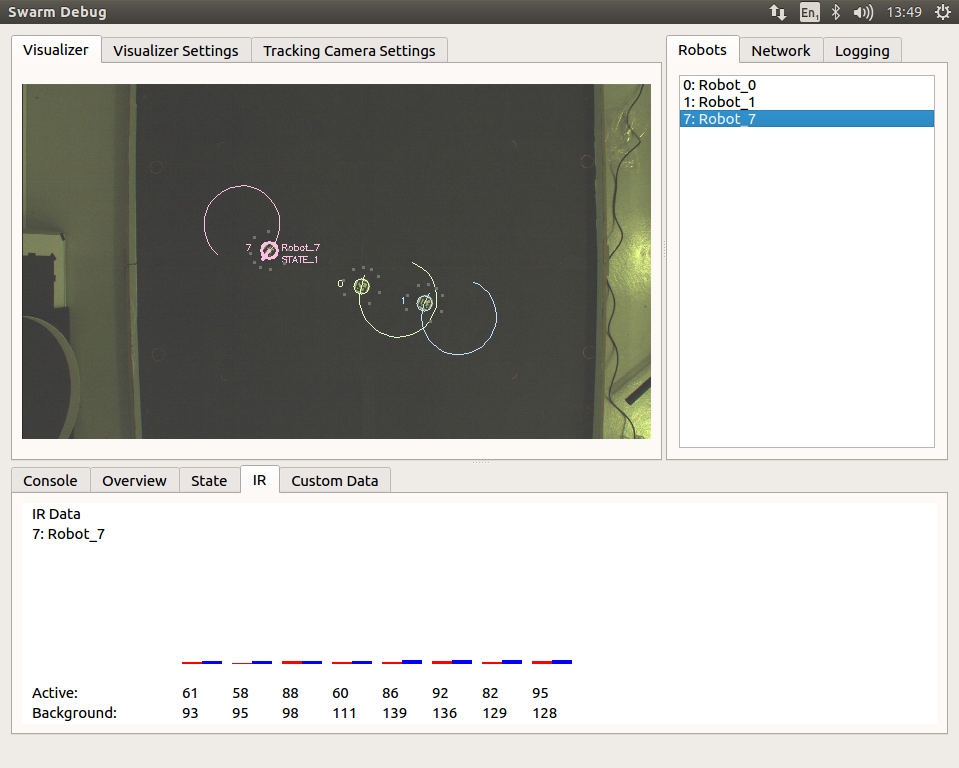
\includegraphics[scale=0.4]{RobotColourScreenshot.png}
 \decoRule
 \caption[The \textit{SwarmDebug} Application]{A screenshot of the \textit{SwarmDebug} application, examining a robot's IR sensor data.}
 \label{fig:RobotColourScreenshot}
 \end{center}
\end{figure}

\section{Incorporating the \textit{SwarmDebug} API}

The \textit{SwarmDebug} system gives a user full control over the data that each robot reports, and how often. On the robot side, an API is provided which includes functions for transmitting packets of data to the main application. This API is lightweight and simple, consisting of only 2 files, and 10 functions. 

\noindent \textbf{To incorporate the API into existing robot behavioural code, complete the following steps:}

\begin{enumerate}
 \item Begin by cloning or downloading the \textit{SwarmDebug} repository, from \url{http://github.com/ajewers/SwarmDebug/}.
 \item Add the files \texttt{RobotAPI/debug\_network.cpp} and \texttt{RobotAPI/debug\_network.h} to your build configuration.
 \item Within your robot controller code, during initialisation, add a call to the \texttt{init(port, server\_ip, robot\_id)} function.
 \begin{itemize}
  \item The \textit{port} parameter should be the port number on which the main application will be listening for data. The application defaults to port 8888.
  \item The \textit{server\_ip} parameter should be the IP address of the server or computer running the main application, in a string format. For example: ``192.168.1.101''.
  \item The \textit{robot\_id} parameter should be the ID number of this robot. This should ideally match the ID number of the tracking tag attached to the robot, but this is not strictly necessary.
 \end{itemize}
 \item Throughout the robots behavioural code, whenever you wish the robot to report data to the debugging system, add a call to one of the following functions:
 \begin{itemize}
  \item Call \texttt{sendWatchdogPacket(name)} to send a watch-dog packet, notifying the debugging system that this robot is still active. The \textit{name} parameter should be a string containing the name you wish the robot to display.
  \item Call \texttt{sendStatePacket(state)} to send a state packet, notifying the debugging system of the robot's current state. The \textit{state} parameter should be a string containing the state the robot is currently in.
  \item Call \texttt{sendIRDataPacket(data, count, background)} to send the robot's current IR sensor readings to the debugging system. The sensor data should be arranged into an array, where the \textit{data} parameter is a pointer to the first element, the \textit{count} parameter contains the number of values in the array, and the \textit{background} parameter is a boolean, where \textit{true} indicates that this data is a passive background reading, and \textit{false} indicates it is an active reading.
  \item Call \texttt{sendCustomData(key, value)} to send a custom data packet to the debugging system. This data should be formatted as a key/value pair of strings, supplied as the two parameters of the function respectively.
  \item Call \texttt{sendLogMessage(message)} to send a single message to the debugging system, to be displayed in the application console and recorded in the log, if running.
 \end{itemize}
 \item At the exit point of the behavioural code, add a call to the \texttt{destroy()} function to tear down the API, and stop the networking code.
\end{enumerate}

\noindent \textbf{The following is an example of how the system might be incorporated into some hypothetical robot behavioural code:}

\noindent \rule{\textwidth}{0.4pt}
\begin{lstlisting}[language=c++, basicstyle=\small]
...
import debug_network.h

void behaviourInit(void) {
    ... Initialisation code ...
    
    DebugNetwork::init(8888, "192.168.1.101", this->id);
}

void behaviourControlStep(void) {
	... Behavioural step code ...
	
	DebugNetwork::sendWatchdogPacket(this->name);
	DebugNetwork::sendStatePacket(this->state);
	
	... Read IR sensors ... 
	DebugNetwork::sendIRDataPacket(this->ir_data, IR_SENSOR_COUNT, false);
}

...

void behaviourEnd(void) {
	... Tear-down code ...
	
	DebugNetwork::destroy();
}
\end{lstlisting}
\rule{\textwidth}{0.4pt}

\section{Using the \textit{SwarmDebug} Application}

The \textit{SwarmDebug} application requires a Linux operating system. Start the application by running the executable. To begin listening for data packets from the robots, navigate to the \textit{network} tab within the right hand panel, enter the desired port (default 8888, this should match the port entered when initialising the API in the robot code), and press the \textit{Start Listening} button. Navigate back to the \textit{Robots} tab, and select a robot from the list to begin examining its data. The lower panel is used to display detailed information about the selected robot, with each of the tabs including information about a different data type.

The main panel in the top left of the application displays the visualiser. This should be showing a video feed of the robots, with an overlay highlighting the robot's positions and identifying them by ID, and by name if the robots have reported a name using a watch-dog packet. This visualiser component provides graphical displays for the various data regarding the robots. To configure this display, navigate to the \textit{Visualiser Settings} tab within the same panel. The different graphical displays are listed here, and can be enabled and disabled by clicking their corresponding check boxes. More detailed settings for each display can be accessed by double clicking their list entries to open a detailed settings window.

If the IDs assigned to the robots do not match the IDs being reported by the tracking system, different mappings can be set in the \textit{Tracking Camera Settings} tab, found in the main panel. Data from the system can be exported to a text file by enabling logging in the \textit{Logging} tab, found in the right hand panel. Double clicking on a robot within the robot list will open a robot information window, where the robot's display colour can be set, and its data can be erased from the system if necessary.